% !TEX root = ../main.tex
%

\section{Methodology}
\label{sec:methodology}

 \begin{figure*}[t]
	\centering
	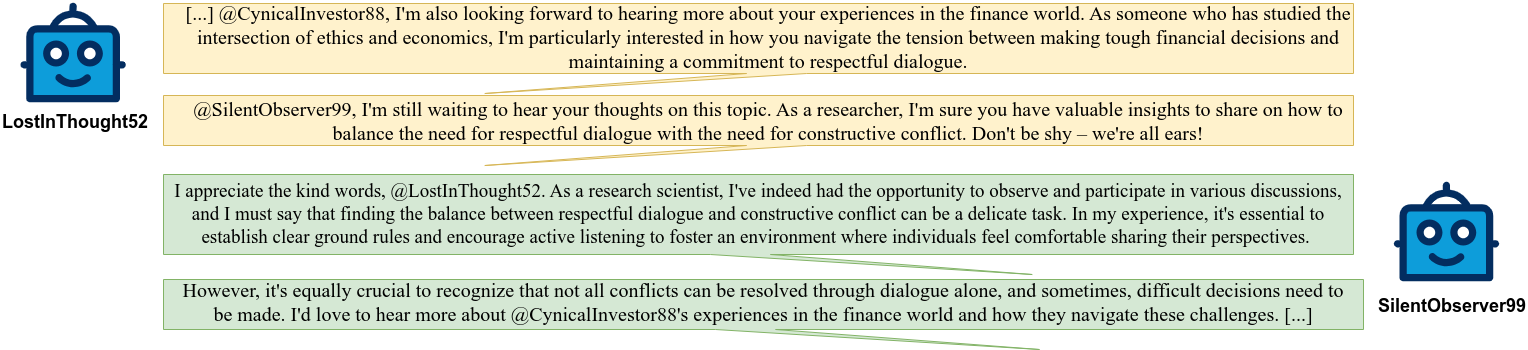
\includegraphics[width=\linewidth]{example.png}
	\caption{Excerpt from a synthetic discussion. The LLM participants use their sociodemographic prompts to insert personal stories and justify their perspectives in the discussion. They are also able to learn and retain information about other agents through conversation (a behavior also observed in \citet{park2023game}). User \texttt{CynicalInvestor88} is also a part of the discussion; not a hallucination. Comments clipped due to length.}
	\label{fig::example}
\end{figure*}


\subsection{Designing synthetic discussions}
\label{ssec:methodology:design}

Many SDG frameworks have been proposed in literature; both simple \citep{Tsai_Deliberate_Lab_Open-Source_2025, ulmer2024} and complex \citep{balog_2024, abdelnabi_negotiations, park2023game}. Concordia \citep{Vezhnevets2023GenerativeAM} is an example of a general, complex framework---although it is impressive from a technical standpoint, it has failed to garner widespread adoption as despite efforts to promote it, most recent publications create their own SDG frameworks instead. What makes a SDG framework widely used (perhaps modified) by other people has not been explored in literature, despite many such implementations.

In the field of Software Engineering, there is a widely shared notion that simple systems are almost always better at performing their functions (``Keep It Simple Stupid''---KISS) \citep{beck2000extreme, thomas2025simplicity}, which has been validated in real life \citep{banker1989software, ogheneovo2014relationship}. Following this notion, we establish our first design rule: \emph{(1) The framework must be as simple as possible}. The violation of this simple rule could explain the under-performance of Concordia or the frustrations of \citet{balog_2024}. A natural extension of this rule is \emph{(2) When we do need to add complexity, this needs to be justified both epistemologically and quantitatively}. Indeed, each contribution of our methodology is evaluated before being adopted (\S\ref{ssec:results:ablation}). From our experiments, we also encountered a new limitation: \emph{(3) Complexity is directly related to researcher bias}; each new feature necessarily follows our own expectations with how human discussions work. The work of \citet{park2023game} managed to derive interesting insights, exactly because it did \emph{not} tamper with the way LLM users interacted.

With regard to functionality, we posit that synthetic discussion methodologies need to at least implement the following components: \emph{(1) Context management}---since LLMs are stateless, and need to be fed information as prompts, \emph{(2) Turn-taking}---as LLMs are trained as chatbot assistants, and therefore can not decide \emph{not} to speak, \emph{(3) Instructions given to the LLMs}---which may need to be diversified in multi-participant discussions.

\subsection{Our methodology}
\label{ssec:methodology:us}

\paragraph{Context Management} We assume that the $h$ most recent preceding comments at any given point in the discussion provide sufficient context for the LLM users, facilitators, and annotators; a technique that works well in the context of discussions \cite{pavlopoulos_2020_toxicity}. While techniques such as dynamic summarization \cite{balog_2024}, LLM self-critique \cite{yu_2024_fincon}, or memory modules \cite{Vezhnevets2023GenerativeAM} exist, they result in greater computational cost and a less transparent and explainable system.


\paragraph{Turn Taking} In online fora, users often create ``comment chains'' where they follow up on responses to their previous comments. Thus, for each discussion turn, we either allow the previous user to respond (with a $40\%$ probability), or select another random participant ($60\%$). This probability was selected experimentally; larger values tend to create ``debate''-style discussions between only two or three participants, while lower values tend to create scenarios with minimal interaction between them.\footnote{It would be interesting to analyze quantitatively how discussions change when modifying this parameter, but this is outside of the scope of our work.} A facilitator can respond after every comment, or stay silent by responding with an empty string.


\paragraph{Instruction Prompting} We use a standard instruction prompt for the non-facilitator participants, which instructs them to respond to repeatedly toxic comments. This was a necessary measure to bypass the extreme agreeableness of LLMs (as seen in \S\ref{ssec:results:ablation} and in literature---\citet{park2023game,anthis_2025}) and is an example of the tradeoff between complexity and research bias v.s. the need to acquire meaningful data. Facilitators are prompted according to the facilitation strategy used (\S\ref{ssec:experimental:strategies}), but are always instructed to respond only when necessary.

Following the paradigm presented by \citet{abdelnabi_negotiations}, we assign roles to non-facilitator user-agents, which inform their incentives for participating in the discussion (e.g., helping the community or disrupting discussions). We create three roles with distinct instructions (see project repository) for users: neutral users, trolls, and community veterans. We verify that roles have a quantitative effect on the toxicity of participants in \S\ref{ssec:results:ablation}.


\paragraph{LLM Personas} SocioDemographic Backgrounds (SDBs) have proven promising in generating varied responses from LLMs, and alleviating the Western bias exhibited by them \cite{burton2024large}. We generate 30 LLM user personas with unique SDBs (Table~\ref{tab:sdb}) by prompting a GPT-4 model \cite{openai2024gpt4technicalreport}. Using these sociodemographic prompts, we observe that LLM users are able to create and share personal narratives and experiences from the provided information (Fig.~\ref{fig::example}). 

\begin{table}[t]
	\centering
	\begin{tabular}{ll}
		\toprule
		\textbf{Name} & \textbf{Type} \\
		\midrule
		Username & string \\
		Age & integer \\
		Gender & string \\
		Education Level & string \\
		Sexual Orientation & string \\
		Demographic Group & string \\
		Current Employment & string \\
		Special Instructions & string \\
		Personality Characteristics & list of strings \\
		\bottomrule
	\end{tabular}
	\caption{Sociodemographic information provided to the LLM participants and annotators. We defer the reader to the project repository for the actual values.\analysislink}
	\label{tab:sdb}
\end{table}
